\documentclass[twoside]{book}

% Packages required by doxygen
\usepackage{fixltx2e}
\usepackage{calc}
\usepackage{doxygen}
\usepackage[export]{adjustbox} % also loads graphicx
\usepackage{graphicx}
\usepackage[utf8]{inputenc}
\usepackage{makeidx}
\usepackage{multicol}
\usepackage{multirow}
\PassOptionsToPackage{warn}{textcomp}
\usepackage{textcomp}
\usepackage[nointegrals]{wasysym}
\usepackage[table]{xcolor}

% Font selection
\usepackage[T1]{fontenc}
\usepackage[scaled=.90]{helvet}
\usepackage{courier}
\usepackage{amssymb}
\usepackage{sectsty}
\renewcommand{\familydefault}{\sfdefault}
\allsectionsfont{%
  \fontseries{bc}\selectfont%
  \color{darkgray}%
}
\renewcommand{\DoxyLabelFont}{%
  \fontseries{bc}\selectfont%
  \color{darkgray}%
}
\newcommand{\+}{\discretionary{\mbox{\scriptsize$\hookleftarrow$}}{}{}}

% Page & text layout
\usepackage{geometry}
\geometry{%
  a4paper,%
  top=2.5cm,%
  bottom=2.5cm,%
  left=2.5cm,%
  right=2.5cm%
}
\tolerance=750
\hfuzz=15pt
\hbadness=750
\setlength{\emergencystretch}{15pt}
\setlength{\parindent}{0cm}
\setlength{\parskip}{3ex plus 2ex minus 2ex}
\makeatletter
\renewcommand{\paragraph}{%
  \@startsection{paragraph}{4}{0ex}{-1.0ex}{1.0ex}{%
    \normalfont\normalsize\bfseries\SS@parafont%
  }%
}
\renewcommand{\subparagraph}{%
  \@startsection{subparagraph}{5}{0ex}{-1.0ex}{1.0ex}{%
    \normalfont\normalsize\bfseries\SS@subparafont%
  }%
}
\makeatother

% Headers & footers
\usepackage{fancyhdr}
\pagestyle{fancyplain}
\fancyhead[LE]{\fancyplain{}{\bfseries\thepage}}
\fancyhead[CE]{\fancyplain{}{}}
\fancyhead[RE]{\fancyplain{}{\bfseries\leftmark}}
\fancyhead[LO]{\fancyplain{}{\bfseries\rightmark}}
\fancyhead[CO]{\fancyplain{}{}}
\fancyhead[RO]{\fancyplain{}{\bfseries\thepage}}
\fancyfoot[LE]{\fancyplain{}{}}
\fancyfoot[CE]{\fancyplain{}{}}
\fancyfoot[RE]{\fancyplain{}{\bfseries\scriptsize Generated by Doxygen }}
\fancyfoot[LO]{\fancyplain{}{\bfseries\scriptsize Generated by Doxygen }}
\fancyfoot[CO]{\fancyplain{}{}}
\fancyfoot[RO]{\fancyplain{}{}}
\renewcommand{\footrulewidth}{0.4pt}
\renewcommand{\chaptermark}[1]{%
  \markboth{#1}{}%
}
\renewcommand{\sectionmark}[1]{%
  \markright{\thesection\ #1}%
}

% Indices & bibliography
\usepackage{natbib}
\usepackage[titles]{tocloft}
\setcounter{tocdepth}{3}
\setcounter{secnumdepth}{5}
\makeindex

% Hyperlinks (required, but should be loaded last)
\usepackage{ifpdf}
\ifpdf
  \usepackage[pdftex,pagebackref=true]{hyperref}
\else
  \usepackage[ps2pdf,pagebackref=true]{hyperref}
\fi
\hypersetup{%
  colorlinks=true,%
  linkcolor=blue,%
  citecolor=blue,%
  unicode%
}

% Custom commands
\newcommand{\clearemptydoublepage}{%
  \newpage{\pagestyle{empty}\cleardoublepage}%
}

\usepackage{caption}
\captionsetup{labelsep=space,justification=centering,font={bf},singlelinecheck=off,skip=4pt,position=top}

%===== C O N T E N T S =====

\begin{document}

% Titlepage & ToC
\hypersetup{pageanchor=false,
             bookmarksnumbered=true,
             pdfencoding=unicode
            }
\pagenumbering{alph}
\begin{titlepage}
\vspace*{7cm}
\begin{center}%
{\Large Transit Simulator and Visualization Project }\\
\vspace*{1cm}
{\large Generated by Doxygen 1.8.13}\\
\end{center}
\end{titlepage}
\clearemptydoublepage
\pagenumbering{roman}
\tableofcontents
\clearemptydoublepage
\pagenumbering{arabic}
\hypersetup{pageanchor=true}

%--- Begin generated contents ---
\chapter{Transit Simulator and Visualization Project}
\label{index}\hypertarget{index}{}\hypertarget{index_intro_sec}{}\section{Introduction}\label{index_intro_sec}
This is the introduction. Hello world! This is Jingyi\textquotesingle{}s first Doxygen file! 
\chapter{Hierarchical Index}
\section{Class Hierarchy}
This inheritance list is sorted roughly, but not completely, alphabetically\+:\begin{DoxyCompactList}
\item \contentsline{section}{Bus}{\pageref{classBus}}{}
\begin{DoxyCompactList}
\item \contentsline{section}{Large\+Bus}{\pageref{classLargeBus}}{}
\item \contentsline{section}{Regular\+Bus}{\pageref{classRegularBus}}{}
\item \contentsline{section}{Small\+Bus}{\pageref{classSmallBus}}{}
\end{DoxyCompactList}
\item \contentsline{section}{Bus\+Factory}{\pageref{classBusFactory}}{}
\item \contentsline{section}{Visualization\+Simulator}{\pageref{classVisualizationSimulator}}{}
\end{DoxyCompactList}

\chapter{Class Index}
\section{Class List}
Here are the classes, structs, unions and interfaces with brief descriptions\+:\begin{DoxyCompactList}
\item\contentsline{section}{\hyperlink{classBus}{Bus} \\*As the description mentioned above, \hyperlink{classBus}{Bus} Factory was created to generate different types of buses. So, in this class, I implimented three different buses categorized by capacity of the bus, small, regular, and large. Small bus will have 30 maximum capacity, regular is assigned with 60 capacity while large can load 90 passengers maximum. The three class all inherited from their parent class, \hyperlink{classBus}{Bus}. Also, they all have on public class, Report, to tell people which type of bus is generated when the simulator is running }{\pageref{classBus}}{}
\item\contentsline{section}{\hyperlink{classBusFactory}{Bus\+Factory} \\*To make the project more releastic, I implemented a new class, \hyperlink{classBus}{Bus} Factory, which can generate different kinds of buses. So far, the needs for different buses types are just reporting different capacity. So, here I used concreate factory method for bus factory. The class basically just generate the bus and use an int parameter to define the type of the buses. When the parameter is set to one, small bus will be generated, regular size will be generated when 2 is assigned to the parameter and leaves value 3 for having large size bus. The value will be assigned randomly to make sure all kinds of buses will appear on the simulator. The process will be applied in visualization\+\_\+simulator }{\pageref{classBusFactory}}{}
\item\contentsline{section}{\hyperlink{classLargeBus}{Large\+Bus} \\*A Small \hyperlink{classBus}{Bus} product, bus size is 90 maximum capacity }{\pageref{classLargeBus}}{}
\item\contentsline{section}{\hyperlink{classRegularBus}{Regular\+Bus} \\*A Small \hyperlink{classBus}{Bus} product, bus size is 60 maximum capacity }{\pageref{classRegularBus}}{}
\item\contentsline{section}{\hyperlink{classSmallBus}{Small\+Bus} \\*A Small \hyperlink{classBus}{Bus} product, bus size is 30 maximum capacity }{\pageref{classSmallBus}}{}
\item\contentsline{section}{\hyperlink{classVisualizationSimulator}{Visualization\+Simulator} \\*The pause functionality mainly rely on Update(). Because, when the simulator is paused, we want the simulator to stop updating. So, by defining the status of pause button (clicked or not clicked), Update() will make a decision to keep updating or pause the process. The similar logic also works for resume functionality. If pause function is called, then un-\/pause it, or pause the function if the pause function is not called }{\pageref{classVisualizationSimulator}}{}
\end{DoxyCompactList}

\chapter{File Index}
\section{File List}
Here is a list of all documented files with brief descriptions\+:\begin{DoxyCompactList}
\item\contentsline{section}{/home/jinxx679/\+Documents/3081/repo-\/jinxx679/project/src/\hyperlink{bus_8cc}{bus.\+cc} }{\pageref{bus_8cc}}{}
\item\contentsline{section}{/home/jinxx679/\+Documents/3081/repo-\/jinxx679/project/src/\hyperlink{bus_8h}{bus.\+h} }{\pageref{bus_8h}}{}
\item\contentsline{section}{/home/jinxx679/\+Documents/3081/repo-\/jinxx679/project/src/\hyperlink{bus__factory_8h}{bus\+\_\+factory.\+h} }{\pageref{bus__factory_8h}}{}
\item\contentsline{section}{/home/jinxx679/\+Documents/3081/repo-\/jinxx679/project/src/{\bfseries mainpage.\+h} }{\pageref{mainpage_8h}}{}
\item\contentsline{section}{/home/jinxx679/\+Documents/3081/repo-\/jinxx679/project/web\+\_\+code/web/{\bfseries visualization\+\_\+simulator.\+h} }{\pageref{visualization__simulator_8h}}{}
\end{DoxyCompactList}

\chapter{Class Documentation}
\hypertarget{classBus}{}\section{Bus Class Reference}
\label{classBus}\index{Bus@{Bus}}


As the description mentioned above, \hyperlink{classBus}{Bus} Factory was created to generate different types of buses. So, in this class, I implimented three different buses categorized by capacity of the bus, small, regular, and large. Small bus will have 30 maximum capacity, regular is assigned with 60 capacity while large can load 90 passengers maximum. The three class all inherited from their parent class, \hyperlink{classBus}{Bus}. Also, they all have on public class, Report, to tell people which type of bus is generated when the simulator is running.  




{\ttfamily \#include $<$bus.\+h$>$}



Inheritance diagram for Bus\+:\nopagebreak
\begin{figure}[H]
\begin{center}
\leavevmode
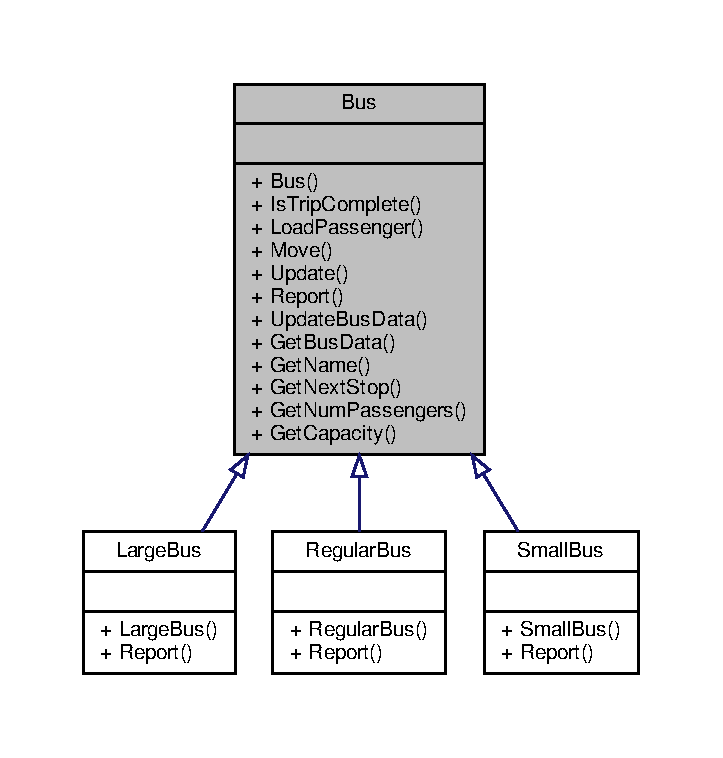
\includegraphics[width=347pt]{classBus__inherit__graph}
\end{center}
\end{figure}


Collaboration diagram for Bus\+:\nopagebreak
\begin{figure}[H]
\begin{center}
\leavevmode
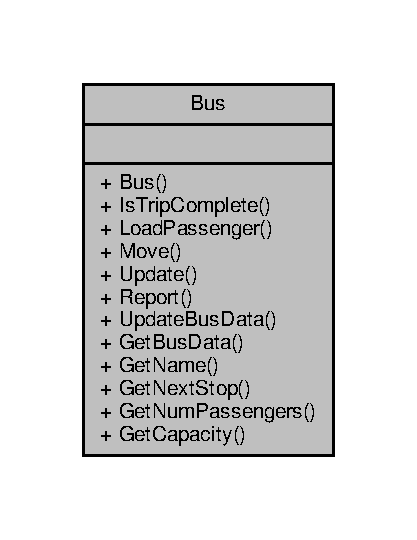
\includegraphics[width=200pt]{classBus__coll__graph}
\end{center}
\end{figure}
\subsection*{Public Member Functions}
\begin{DoxyCompactItemize}
\item 
\mbox{\Hypertarget{classBus_aa28c3c318b6993f3a3aebf211daa9217}\label{classBus_aa28c3c318b6993f3a3aebf211daa9217}} 
{\bfseries Bus} (std\+::string name, Route $\ast$out, Route $\ast$in, int capacity=60, double speed=1)
\item 
\mbox{\Hypertarget{classBus_a9c64b0801bf589f121fb0598b70a99b4}\label{classBus_a9c64b0801bf589f121fb0598b70a99b4}} 
bool {\bfseries Is\+Trip\+Complete} ()
\item 
\mbox{\Hypertarget{classBus_ac3f1c523bc4f97bc8ada8dc488ab3484}\label{classBus_ac3f1c523bc4f97bc8ada8dc488ab3484}} 
bool {\bfseries Load\+Passenger} (Passenger $\ast$)
\item 
\mbox{\Hypertarget{classBus_a5e667186d6db0916ebab0e4eff3312c8}\label{classBus_a5e667186d6db0916ebab0e4eff3312c8}} 
bool {\bfseries Move} ()
\item 
\mbox{\Hypertarget{classBus_a9896f74f16966f7621d0dfafff0ec6b4}\label{classBus_a9896f74f16966f7621d0dfafff0ec6b4}} 
void {\bfseries Update} ()
\item 
\mbox{\Hypertarget{classBus_a4e50209dde52bff3de231c8259b38982}\label{classBus_a4e50209dde52bff3de231c8259b38982}} 
virtual void {\bfseries Report} (std\+::ostream \&)
\item 
\mbox{\Hypertarget{classBus_a38b7ee7b13b3438894e914a6933a6f44}\label{classBus_a38b7ee7b13b3438894e914a6933a6f44}} 
void {\bfseries Update\+Bus\+Data} ()
\item 
\mbox{\Hypertarget{classBus_aee8d077fc426b73942dec2564b5d066a}\label{classBus_aee8d077fc426b73942dec2564b5d066a}} 
Bus\+Data {\bfseries Get\+Bus\+Data} () const
\item 
\mbox{\Hypertarget{classBus_a2143b0563ad48b1b67e114d1ba5342ca}\label{classBus_a2143b0563ad48b1b67e114d1ba5342ca}} 
std\+::string {\bfseries Get\+Name} () const
\item 
\mbox{\Hypertarget{classBus_a6068e9801c6da152f05e40eb26e80b02}\label{classBus_a6068e9801c6da152f05e40eb26e80b02}} 
Stop $\ast$ {\bfseries Get\+Next\+Stop} () const
\item 
\mbox{\Hypertarget{classBus_a346aaa56030d4707886e1db8181e8b55}\label{classBus_a346aaa56030d4707886e1db8181e8b55}} 
size\+\_\+t {\bfseries Get\+Num\+Passengers} () const
\item 
\mbox{\Hypertarget{classBus_a3a1f68e9e2548f981d0150901918922c}\label{classBus_a3a1f68e9e2548f981d0150901918922c}} 
int {\bfseries Get\+Capacity} () const
\end{DoxyCompactItemize}


\subsection{Detailed Description}
As the description mentioned above, \hyperlink{classBus}{Bus} Factory was created to generate different types of buses. So, in this class, I implimented three different buses categorized by capacity of the bus, small, regular, and large. Small bus will have 30 maximum capacity, regular is assigned with 60 capacity while large can load 90 passengers maximum. The three class all inherited from their parent class, \hyperlink{classBus}{Bus}. Also, they all have on public class, Report, to tell people which type of bus is generated when the simulator is running. 

The documentation for this class was generated from the following files\+:\begin{DoxyCompactItemize}
\item 
/home/jinxx679/\+Documents/3081/repo-\/jinxx679/project/src/\hyperlink{bus_8h}{bus.\+h}\item 
/home/jinxx679/\+Documents/3081/repo-\/jinxx679/project/src/\hyperlink{bus_8cc}{bus.\+cc}\end{DoxyCompactItemize}

\hypertarget{classBusFactory}{}\section{Bus\+Factory Class Reference}
\label{classBusFactory}\index{Bus\+Factory@{Bus\+Factory}}


To make the project more releastic, I implemented a new class, \hyperlink{classBus}{Bus} Factory, which can generate different kinds of buses. So far, the needs for different buses types are just reporting different capacity. So, here I used concreate factory method for bus factory. The class basically just generate the bus and use an int parameter to define the type of the buses. When the parameter is set to one, small bus will be generated, regular size will be generated when 2 is assigned to the parameter and leaves value 3 for having large size bus. The value will be assigned randomly to make sure all kinds of buses will appear on the simulator. The process will be applied in visualization\+\_\+simulator.  




{\ttfamily \#include $<$bus\+\_\+factory.\+h$>$}



Collaboration diagram for Bus\+Factory\+:\nopagebreak
\begin{figure}[H]
\begin{center}
\leavevmode
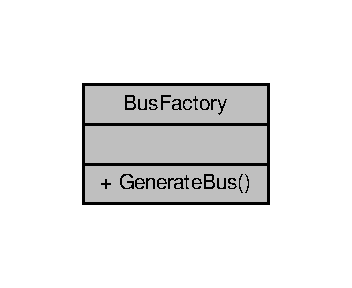
\includegraphics[width=169pt]{classBusFactory__coll__graph}
\end{center}
\end{figure}
\subsection*{Public Member Functions}
\begin{DoxyCompactItemize}
\item 
\mbox{\Hypertarget{classBusFactory_a102f9f2e3090f076196e9e1c67ff32ba}\label{classBusFactory_a102f9f2e3090f076196e9e1c67ff32ba}} 
\hyperlink{classBus}{Bus} $\ast$ {\bfseries Generate\+Bus} (std\+::string name, Route $\ast$out, Route $\ast$in, int bus\+Type, double speed=1)
\end{DoxyCompactItemize}


\subsection{Detailed Description}
To make the project more releastic, I implemented a new class, \hyperlink{classBus}{Bus} Factory, which can generate different kinds of buses. So far, the needs for different buses types are just reporting different capacity. So, here I used concreate factory method for bus factory. The class basically just generate the bus and use an int parameter to define the type of the buses. When the parameter is set to one, small bus will be generated, regular size will be generated when 2 is assigned to the parameter and leaves value 3 for having large size bus. The value will be assigned randomly to make sure all kinds of buses will appear on the simulator. The process will be applied in visualization\+\_\+simulator. 

The documentation for this class was generated from the following files\+:\begin{DoxyCompactItemize}
\item 
/home/jinxx679/\+Documents/3081/repo-\/jinxx679/project/src/\hyperlink{bus__factory_8h}{bus\+\_\+factory.\+h}\item 
/home/jinxx679/\+Documents/3081/repo-\/jinxx679/project/src/bus\+\_\+factory.\+cc\end{DoxyCompactItemize}

\hypertarget{classLargeBus}{}\section{Large\+Bus Class Reference}
\label{classLargeBus}\index{Large\+Bus@{Large\+Bus}}


A Small \hyperlink{classBus}{Bus} product, bus size is 90 maximum capacity.  




{\ttfamily \#include $<$bus.\+h$>$}



Inheritance diagram for Large\+Bus\+:\nopagebreak
\begin{figure}[H]
\begin{center}
\leavevmode
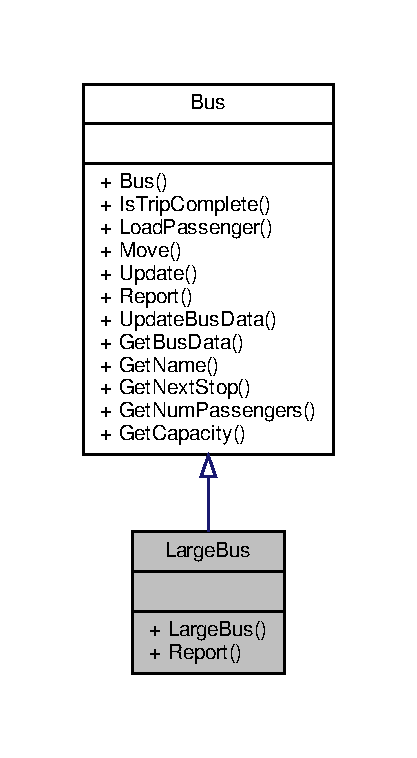
\includegraphics[width=200pt]{classLargeBus__inherit__graph}
\end{center}
\end{figure}


Collaboration diagram for Large\+Bus\+:\nopagebreak
\begin{figure}[H]
\begin{center}
\leavevmode
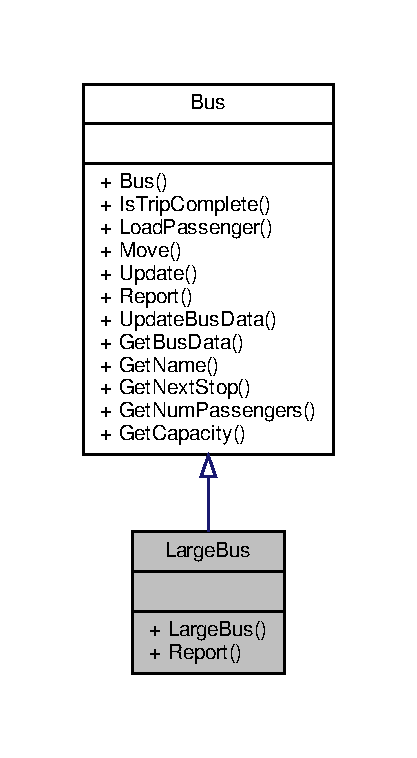
\includegraphics[width=200pt]{classLargeBus__coll__graph}
\end{center}
\end{figure}
\subsection*{Public Member Functions}
\begin{DoxyCompactItemize}
\item 
\mbox{\Hypertarget{classLargeBus_ae1756756d1dbb8db83b4887136e21686}\label{classLargeBus_ae1756756d1dbb8db83b4887136e21686}} 
{\bfseries Large\+Bus} (std\+::string name, Route $\ast$out, Route $\ast$in, double speed=1)
\item 
\mbox{\Hypertarget{classLargeBus_a4e20f9c3199c1099f653f755b618ccea}\label{classLargeBus_a4e20f9c3199c1099f653f755b618ccea}} 
void {\bfseries Report} (std\+::ostream \&) override
\end{DoxyCompactItemize}


\subsection{Detailed Description}
A Small \hyperlink{classBus}{Bus} product, bus size is 90 maximum capacity. 

The documentation for this class was generated from the following files\+:\begin{DoxyCompactItemize}
\item 
/home/jinxx679/\+Documents/3081/repo-\/jinxx679/project/src/\hyperlink{bus_8h}{bus.\+h}\item 
/home/jinxx679/\+Documents/3081/repo-\/jinxx679/project/src/\hyperlink{bus_8cc}{bus.\+cc}\end{DoxyCompactItemize}

\hypertarget{classRegularBus}{}\section{Regular\+Bus Class Reference}
\label{classRegularBus}\index{Regular\+Bus@{Regular\+Bus}}


A Small \hyperlink{classBus}{Bus} product, bus size is 60 maximum capacity.  




{\ttfamily \#include $<$bus.\+h$>$}



Inheritance diagram for Regular\+Bus\+:\nopagebreak
\begin{figure}[H]
\begin{center}
\leavevmode
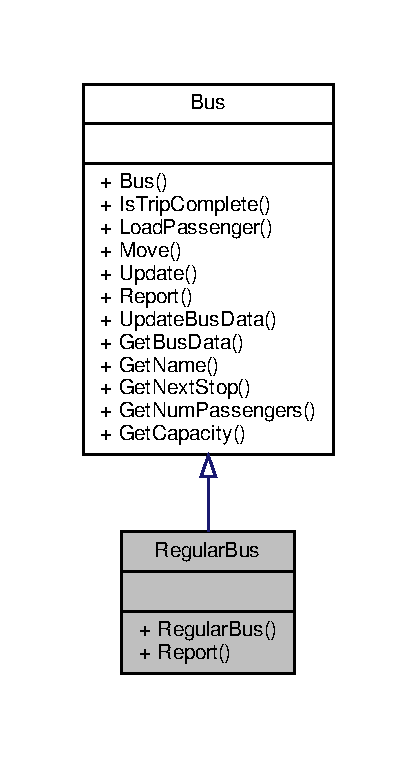
\includegraphics[width=200pt]{classRegularBus__inherit__graph}
\end{center}
\end{figure}


Collaboration diagram for Regular\+Bus\+:\nopagebreak
\begin{figure}[H]
\begin{center}
\leavevmode
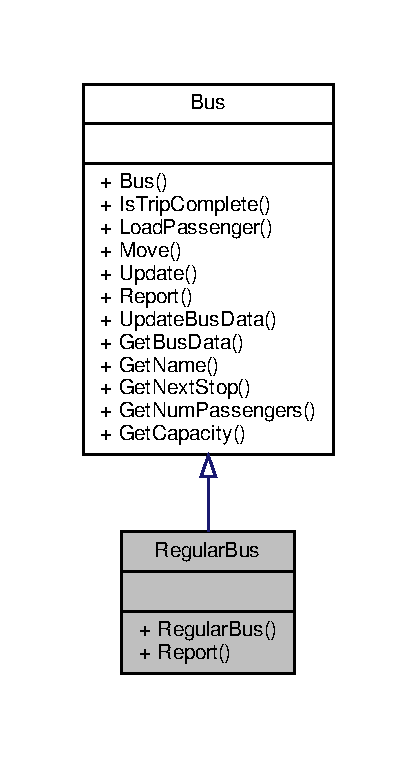
\includegraphics[width=200pt]{classRegularBus__coll__graph}
\end{center}
\end{figure}
\subsection*{Public Member Functions}
\begin{DoxyCompactItemize}
\item 
\mbox{\Hypertarget{classRegularBus_aae4a0754bc23e8d3ac1f701172c4d8a0}\label{classRegularBus_aae4a0754bc23e8d3ac1f701172c4d8a0}} 
{\bfseries Regular\+Bus} (std\+::string name, Route $\ast$out, Route $\ast$in, double speed=1)
\item 
\mbox{\Hypertarget{classRegularBus_a1c8e52afd8ba3cc1f6bf251e9cb10e5f}\label{classRegularBus_a1c8e52afd8ba3cc1f6bf251e9cb10e5f}} 
void {\bfseries Report} (std\+::ostream \&) override
\end{DoxyCompactItemize}


\subsection{Detailed Description}
A Small \hyperlink{classBus}{Bus} product, bus size is 60 maximum capacity. 

The documentation for this class was generated from the following files\+:\begin{DoxyCompactItemize}
\item 
/home/jinxx679/\+Documents/3081/repo-\/jinxx679/project/src/\hyperlink{bus_8h}{bus.\+h}\item 
/home/jinxx679/\+Documents/3081/repo-\/jinxx679/project/src/\hyperlink{bus_8cc}{bus.\+cc}\end{DoxyCompactItemize}

\hypertarget{classSmallBus}{}\section{Small\+Bus Class Reference}
\label{classSmallBus}\index{Small\+Bus@{Small\+Bus}}


A Small \hyperlink{classBus}{Bus} product, bus size is 30 maximum capacity.  




{\ttfamily \#include $<$bus.\+h$>$}



Inheritance diagram for Small\+Bus\+:\nopagebreak
\begin{figure}[H]
\begin{center}
\leavevmode
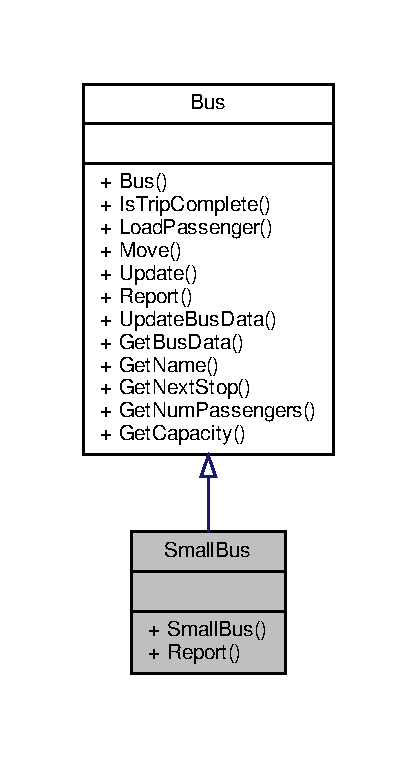
\includegraphics[width=200pt]{classSmallBus__inherit__graph}
\end{center}
\end{figure}


Collaboration diagram for Small\+Bus\+:\nopagebreak
\begin{figure}[H]
\begin{center}
\leavevmode
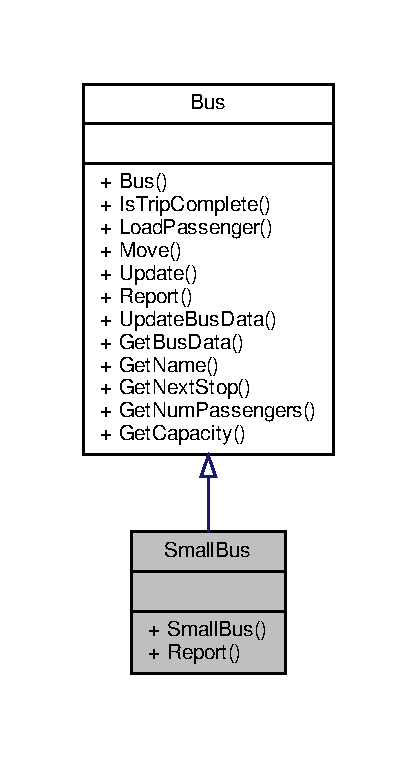
\includegraphics[width=200pt]{classSmallBus__coll__graph}
\end{center}
\end{figure}
\subsection*{Public Member Functions}
\begin{DoxyCompactItemize}
\item 
\mbox{\Hypertarget{classSmallBus_a44623f798fe5ca47c6cf2ffa1276e92e}\label{classSmallBus_a44623f798fe5ca47c6cf2ffa1276e92e}} 
{\bfseries Small\+Bus} (std\+::string name, Route $\ast$out, Route $\ast$in, double speed=1)
\item 
\mbox{\Hypertarget{classSmallBus_a5759f6dd8c3738962730b6f0e28a9c05}\label{classSmallBus_a5759f6dd8c3738962730b6f0e28a9c05}} 
void {\bfseries Report} (std\+::ostream \&) override
\end{DoxyCompactItemize}


\subsection{Detailed Description}
A Small \hyperlink{classBus}{Bus} product, bus size is 30 maximum capacity. 

The documentation for this class was generated from the following file\+:\begin{DoxyCompactItemize}
\item 
/home/jinxx679/\+Documents/3081/repo-\/jinxx679/project/src/\hyperlink{bus_8h}{bus.\+h}\end{DoxyCompactItemize}

\hypertarget{classVisualizationSimulator}{}\section{Visualization\+Simulator Class Reference}
\label{classVisualizationSimulator}\index{Visualization\+Simulator@{Visualization\+Simulator}}


The pause functionality mainly rely on Update(). Because, when the simulator is paused, we want the simulator to stop updating. So, by defining the status of pause button (clicked or not clicked), Update() will make a decision to keep updating or pause the process. The similar logic also works for resume functionality. If pause function is called, then un-\/pause it, or pause the function if the pause function is not called.  




{\ttfamily \#include $<$visualization\+\_\+simulator.\+h$>$}



Collaboration diagram for Visualization\+Simulator\+:\nopagebreak
\begin{figure}[H]
\begin{center}
\leavevmode
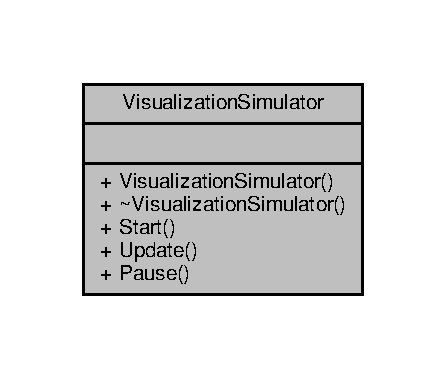
\includegraphics[width=214pt]{classVisualizationSimulator__coll__graph}
\end{center}
\end{figure}
\subsection*{Public Member Functions}
\begin{DoxyCompactItemize}
\item 
\mbox{\Hypertarget{classVisualizationSimulator_a6081cd133454d886ed412f44ad9e8237}\label{classVisualizationSimulator_a6081cd133454d886ed412f44ad9e8237}} 
{\bfseries Visualization\+Simulator} (Web\+Interface $\ast$, Config\+Manager $\ast$)
\item 
\mbox{\Hypertarget{classVisualizationSimulator_abbf0bc7c2913dd690900578e17a4cdcb}\label{classVisualizationSimulator_abbf0bc7c2913dd690900578e17a4cdcb}} 
void {\bfseries Start} (const std\+::vector$<$ int $>$ \&, const int \&)
\item 
\mbox{\Hypertarget{classVisualizationSimulator_a211b13dd71e679f58bd645089ae10319}\label{classVisualizationSimulator_a211b13dd71e679f58bd645089ae10319}} 
void {\bfseries Update} ()
\item 
\mbox{\Hypertarget{classVisualizationSimulator_a7f0452e9e371a1bf2d8afb0873771da4}\label{classVisualizationSimulator_a7f0452e9e371a1bf2d8afb0873771da4}} 
void {\bfseries Pause} ()
\end{DoxyCompactItemize}


\subsection{Detailed Description}
The pause functionality mainly rely on Update(). Because, when the simulator is paused, we want the simulator to stop updating. So, by defining the status of pause button (clicked or not clicked), Update() will make a decision to keep updating or pause the process. The similar logic also works for resume functionality. If pause function is called, then un-\/pause it, or pause the function if the pause function is not called. 

The documentation for this class was generated from the following file\+:\begin{DoxyCompactItemize}
\item 
/home/jinxx679/\+Documents/3081/repo-\/jinxx679/project/web\+\_\+code/web/visualization\+\_\+simulator.\+h\end{DoxyCompactItemize}

\chapter{File Documentation}
\hypertarget{bus_8cc}{}\section{/home/jinxx679/\+Documents/3081/repo-\/jinxx679/project/src/bus.cc File Reference}
\label{bus_8cc}\index{/home/jinxx679/\+Documents/3081/repo-\/jinxx679/project/src/bus.\+cc@{/home/jinxx679/\+Documents/3081/repo-\/jinxx679/project/src/bus.\+cc}}
{\ttfamily \#include \char`\"{}src/bus.\+h\char`\"{}}\newline
{\ttfamily \#include \char`\"{}src/passenger.\+h\char`\"{}}\newline
{\ttfamily \#include \char`\"{}src/stop.\+h\char`\"{}}\newline
Include dependency graph for bus.\+cc\+:\nopagebreak
\begin{figure}[H]
\begin{center}
\leavevmode
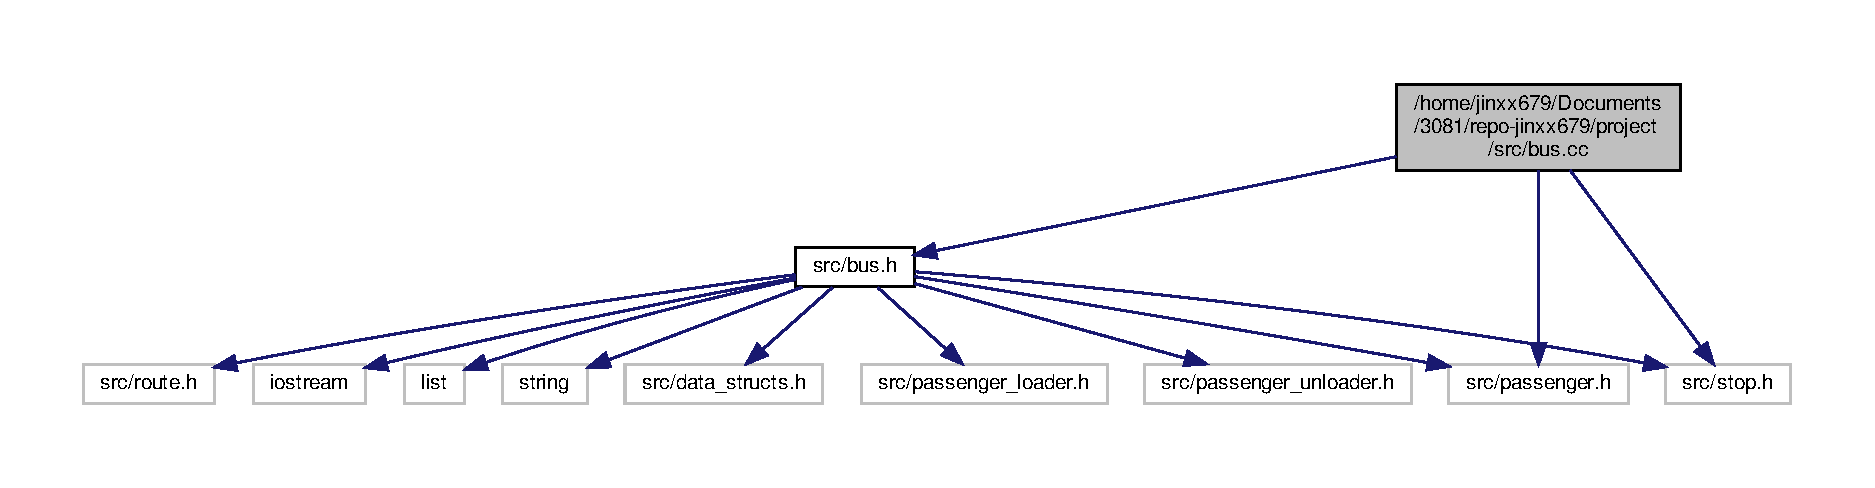
\includegraphics[width=350pt]{bus_8cc__incl}
\end{center}
\end{figure}


\subsection{Detailed Description}
\begin{DoxyCopyright}{Copyright}
2019 3081 Staff, All rights reserved. 
\end{DoxyCopyright}

\hypertarget{bus_8h}{}\section{/home/jinxx679/\+Documents/3081/repo-\/jinxx679/project/src/bus.h File Reference}
\label{bus_8h}\index{/home/jinxx679/\+Documents/3081/repo-\/jinxx679/project/src/bus.\+h@{/home/jinxx679/\+Documents/3081/repo-\/jinxx679/project/src/bus.\+h}}
{\ttfamily \#include $<$iostream$>$}\newline
{\ttfamily \#include $<$list$>$}\newline
{\ttfamily \#include $<$string$>$}\newline
{\ttfamily \#include \char`\"{}src/data\+\_\+structs.\+h\char`\"{}}\newline
{\ttfamily \#include \char`\"{}src/passenger.\+h\char`\"{}}\newline
{\ttfamily \#include \char`\"{}src/passenger\+\_\+loader.\+h\char`\"{}}\newline
{\ttfamily \#include \char`\"{}src/passenger\+\_\+unloader.\+h\char`\"{}}\newline
{\ttfamily \#include \char`\"{}src/route.\+h\char`\"{}}\newline
{\ttfamily \#include \char`\"{}src/stop.\+h\char`\"{}}\newline
Include dependency graph for bus.\+h\+:\nopagebreak
\begin{figure}[H]
\begin{center}
\leavevmode
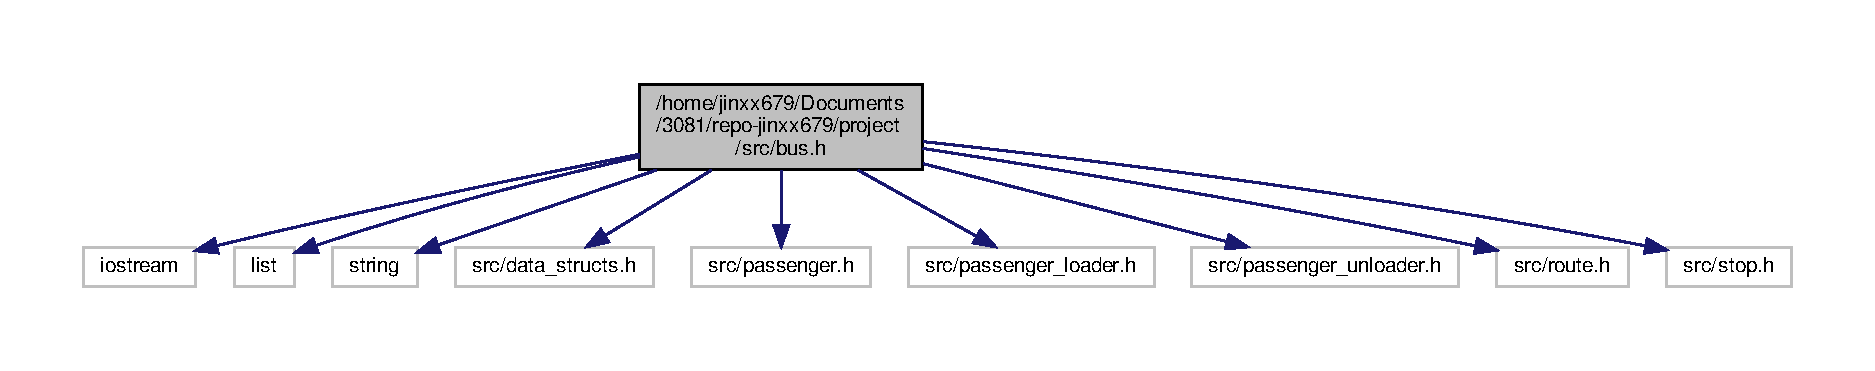
\includegraphics[width=350pt]{bus_8h__incl}
\end{center}
\end{figure}
This graph shows which files directly or indirectly include this file\+:
\nopagebreak
\begin{figure}[H]
\begin{center}
\leavevmode
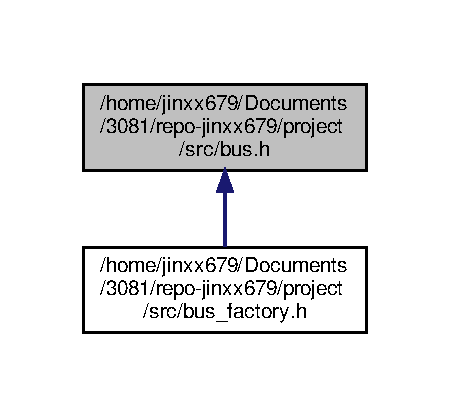
\includegraphics[width=216pt]{bus_8h__dep__incl}
\end{center}
\end{figure}
\subsection*{Classes}
\begin{DoxyCompactItemize}
\item 
class \hyperlink{classBus}{Bus}
\begin{DoxyCompactList}\small\item\em As the description mentioned above, \hyperlink{classBus}{Bus} Factory was created to generate different types of buses. So, in this class, I implimented three different buses categorized by capacity of the bus, small, regular, and large. Small bus will have 30 maximum capacity, regular is assigned with 60 capacity while large can load 90 passengers maximum. The three class all inherited from their parent class, \hyperlink{classBus}{Bus}. Also, they all have on public class, Report, to tell people which type of bus is generated when the simulator is running. \end{DoxyCompactList}\item 
class \hyperlink{classSmallBus}{Small\+Bus}
\begin{DoxyCompactList}\small\item\em A Small \hyperlink{classBus}{Bus} product, bus size is 30 maximum capacity. \end{DoxyCompactList}\item 
class \hyperlink{classRegularBus}{Regular\+Bus}
\begin{DoxyCompactList}\small\item\em A Small \hyperlink{classBus}{Bus} product, bus size is 60 maximum capacity. \end{DoxyCompactList}\item 
class \hyperlink{classLargeBus}{Large\+Bus}
\begin{DoxyCompactList}\small\item\em A Small \hyperlink{classBus}{Bus} product, bus size is 90 maximum capacity. \end{DoxyCompactList}\end{DoxyCompactItemize}


\subsection{Detailed Description}
\begin{DoxyCopyright}{Copyright}
2019 3081 Staff, All rights reserved. 
\end{DoxyCopyright}

\hypertarget{bus__factory_8h}{}\section{/home/jinxx679/\+Documents/3081/repo-\/jinxx679/project/src/bus\+\_\+factory.h File Reference}
\label{bus__factory_8h}\index{/home/jinxx679/\+Documents/3081/repo-\/jinxx679/project/src/bus\+\_\+factory.\+h@{/home/jinxx679/\+Documents/3081/repo-\/jinxx679/project/src/bus\+\_\+factory.\+h}}
{\ttfamily \#include $<$vector$>$}\newline
{\ttfamily \#include $<$random$>$}\newline
{\ttfamily \#include \char`\"{}src/bus.\+h\char`\"{}}\newline
Include dependency graph for bus\+\_\+factory.\+h\+:\nopagebreak
\begin{figure}[H]
\begin{center}
\leavevmode
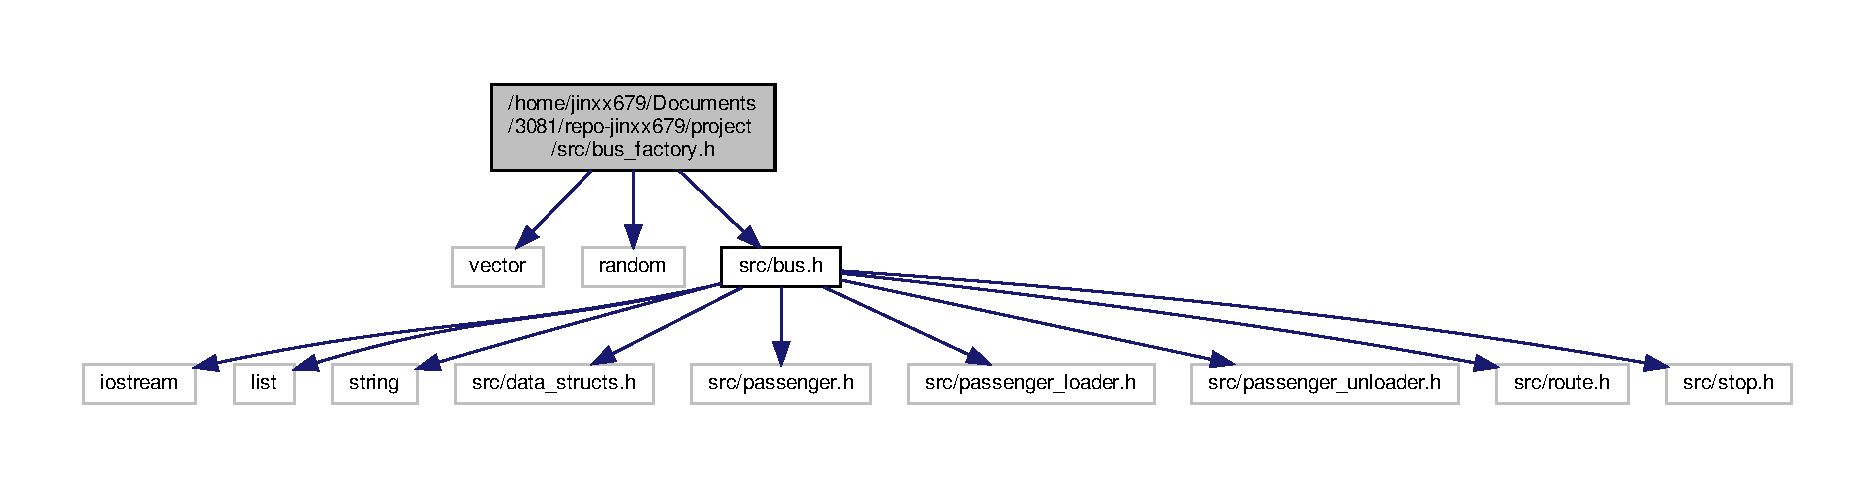
\includegraphics[width=350pt]{bus__factory_8h__incl}
\end{center}
\end{figure}
\subsection*{Classes}
\begin{DoxyCompactItemize}
\item 
class \hyperlink{classBusFactory}{Bus\+Factory}
\begin{DoxyCompactList}\small\item\em To make the project more releastic, I implemented a new class, \hyperlink{classBus}{Bus} Factory, which can generate different kinds of buses. So far, the needs for different buses types are just reporting different capacity. So, here I used concreate factory method for bus factory. The class basically just generate the bus and use an int parameter to define the type of the buses. When the parameter is set to one, small bus will be generated, regular size will be generated when 2 is assigned to the parameter and leaves value 3 for having large size bus. The value will be assigned randomly to make sure all kinds of buses will appear on the simulator. The process will be applied in visualization\+\_\+simulator. \end{DoxyCompactList}\end{DoxyCompactItemize}


\subsection{Detailed Description}
\begin{DoxyCopyright}{Copyright}
2019 3081 Staff, All rights reserved. 
\end{DoxyCopyright}

%--- End generated contents ---

% Index
\backmatter
\newpage
\phantomsection
\clearemptydoublepage
\addcontentsline{toc}{chapter}{Index}
\printindex

\end{document}
